\begin{frame}{$\chi_{b1,2}(3P) \to \ThreeS$ fit model}
\begin{columns}[T]
\column{.5\textwidth}
  \centering
  \setlength{\unitlength}{1mm}
  \begin{picture}(50,80)
      %
    \put(0,0){
      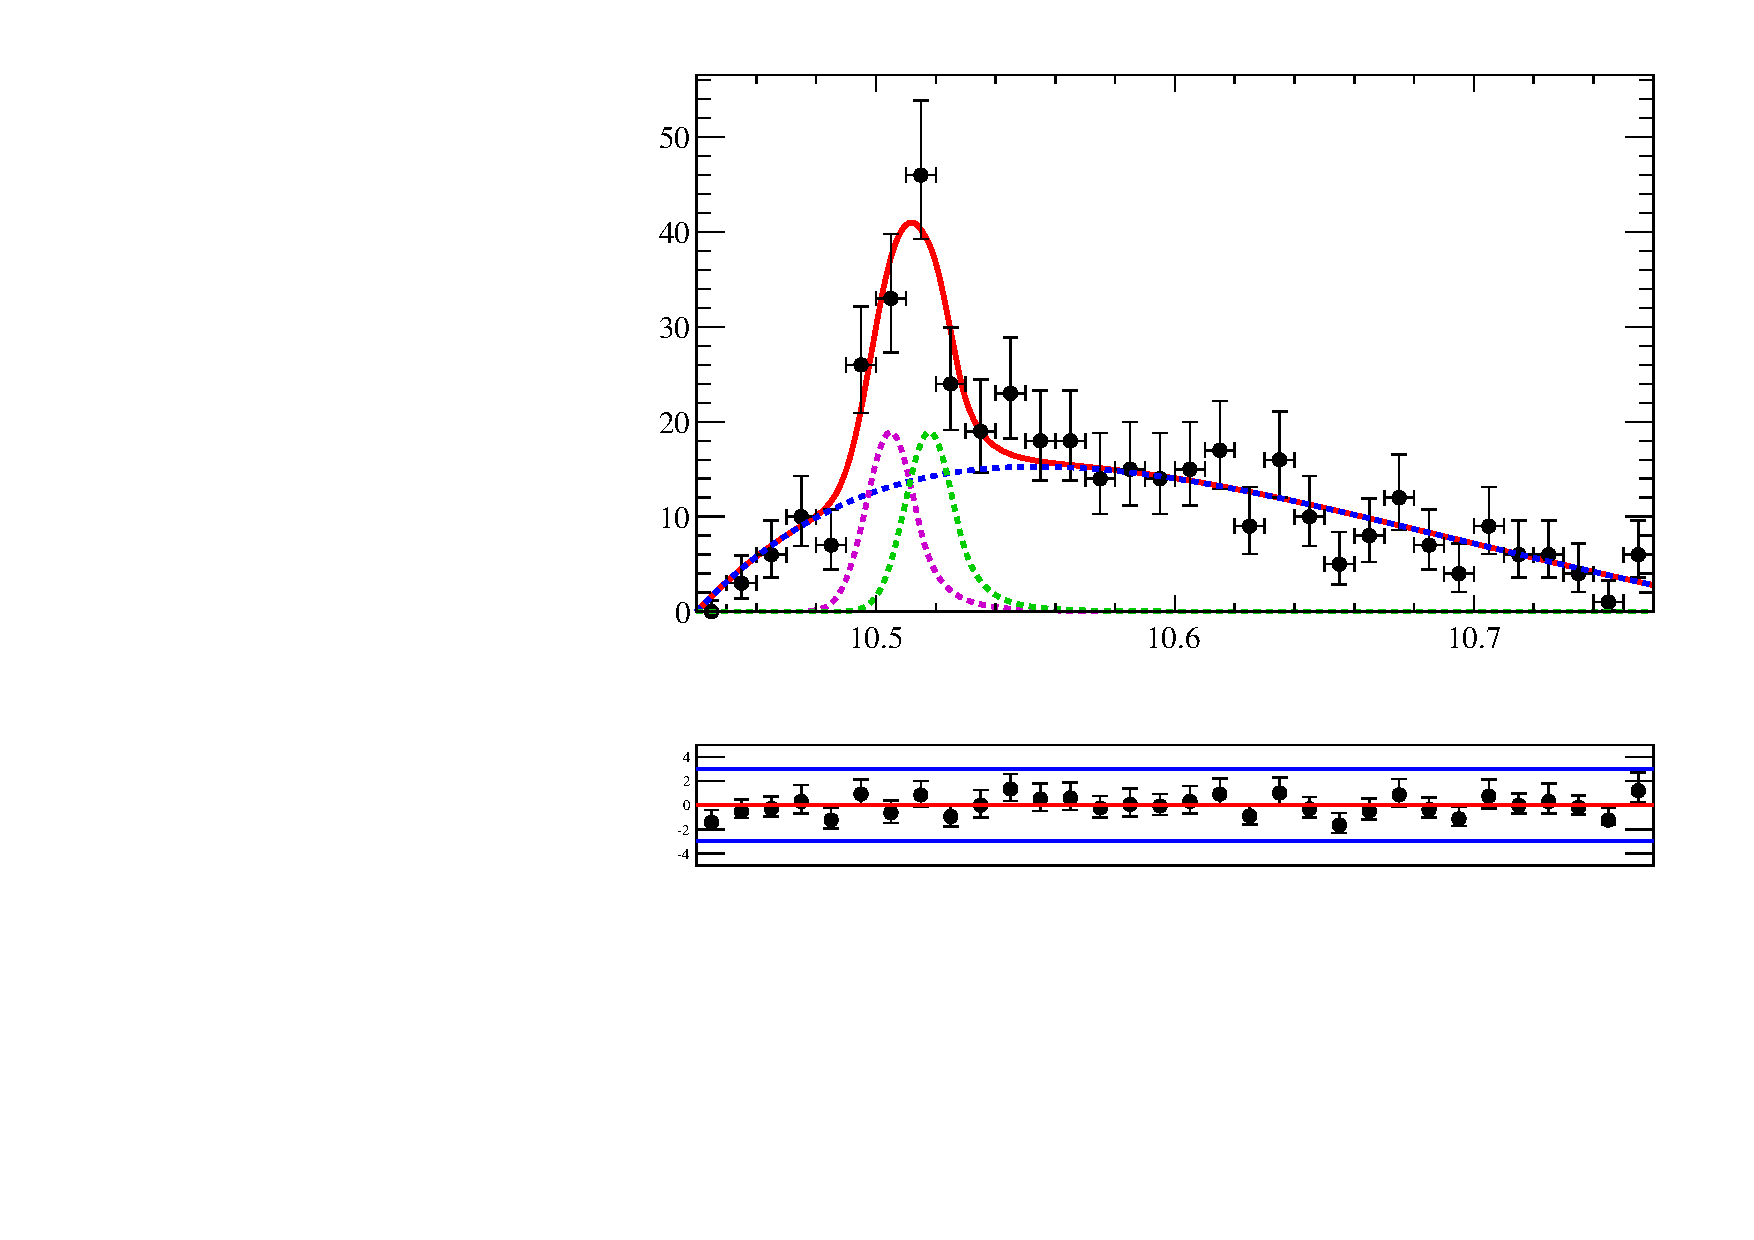
\includegraphics[width=50mm, height=40mm]{chib3s-fit/f2012_fix_27_None}
    }
    
    \put(0,40){
      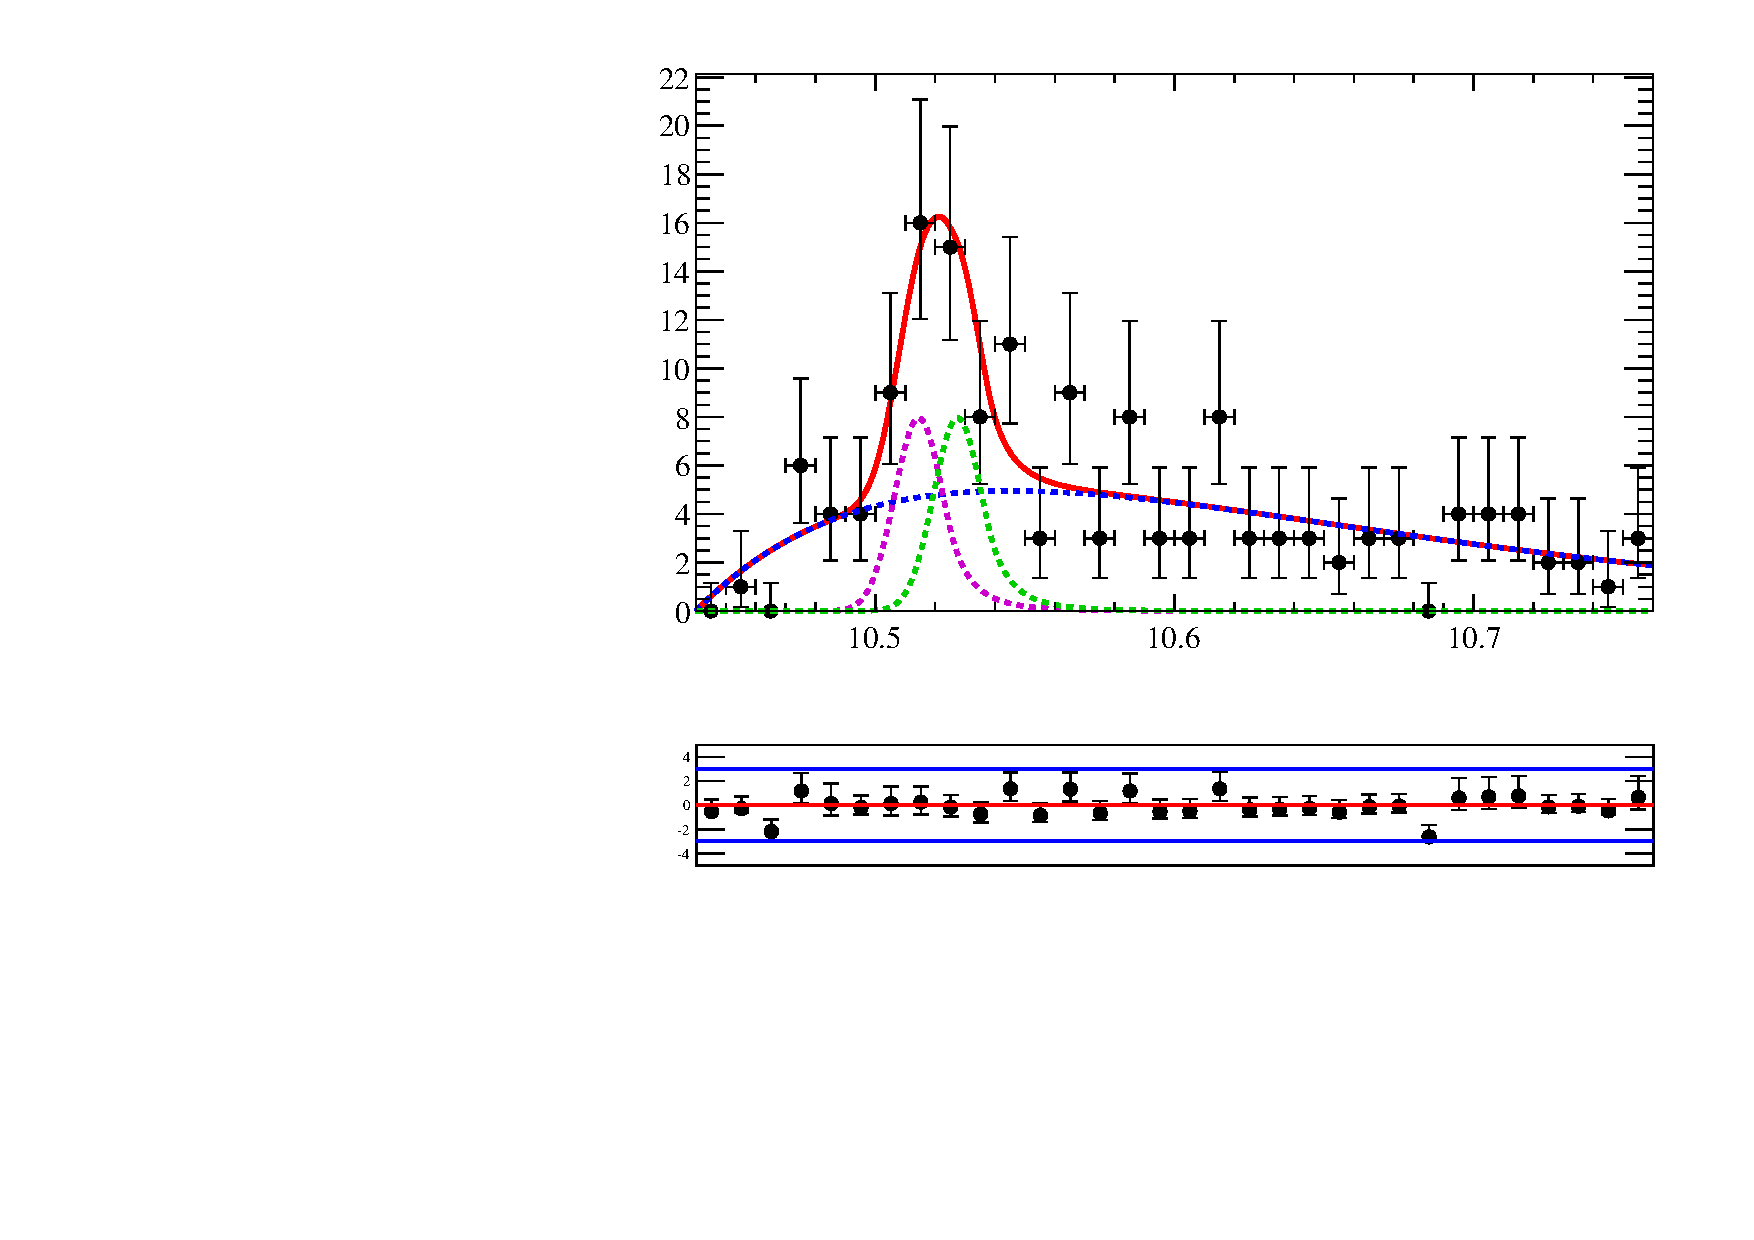
\includegraphics[width=50mm, height=40mm]{chib3s-fit/f2011_fix_27_None}
    }

    \put(0,15){\tiny \begin{sideways}Candidates/(20\mevcc)\end{sideways}}
    \put(2,9.5){\tiny $m_{\mumu \gamma} - m_{\mumu} + 10.3552 \left[\gevcc\right]$}
    \put(25,30){$\sqrt{s} = 8 \gev$}
    \put(20,25){\tiny $p_T(\Y3S) > 27 \gevc$}    
    
    \put(0,55){\tiny \begin{sideways}Candidates/(20\mevcc)\end{sideways}}
    \put(2, 49.5){\tiny $m_{\mumu \gamma} - m_{\mumu} + 10.3552 \left[\gevcc\right]$}
    \put(25,70){$\sqrt{s} = 7 \gev$}     
    \put(20,65){\tiny $p_T(\Y3S) > 27 \gevc$}        
    %\graphpaper[2](0,0)(50, 40)        
  \end{picture}
\column{.5\textwidth}
\begin{itemize}
\item 2 Crystal Ball for each of $\chi_{b1,2}(3P)$ signal.
\item Product of exponential and linear compination of basic Bernstein polinomials  for combinatorial background.
\end{itemize}
\end{columns}
\end{frame}
